\chapter{導論}
\label{c:1}

%==========================================================================================
\section{導論}
%首先界定您的研究問題的研究領域並說明此領域在廣度上的重要性。
卷積神經網路為近年來在物件偵測及辨識度上表現最為突出的深度學習架構,本論文中,我們選定現在在物件偵測上效能與辨識度最高的YOLO(You Only Look Once)作為解析的範本,介紹卷積神經網路的運作過程,比較其他種物件偵測的演算法,拆解YOLO內部的運作過程,探討YOLO能夠領先於其他演算法的關鍵原因,並改善其只能在C++或python中使用之限制,改為在HTML上使用。
\\
\begin{figure}[H]
  \centering
    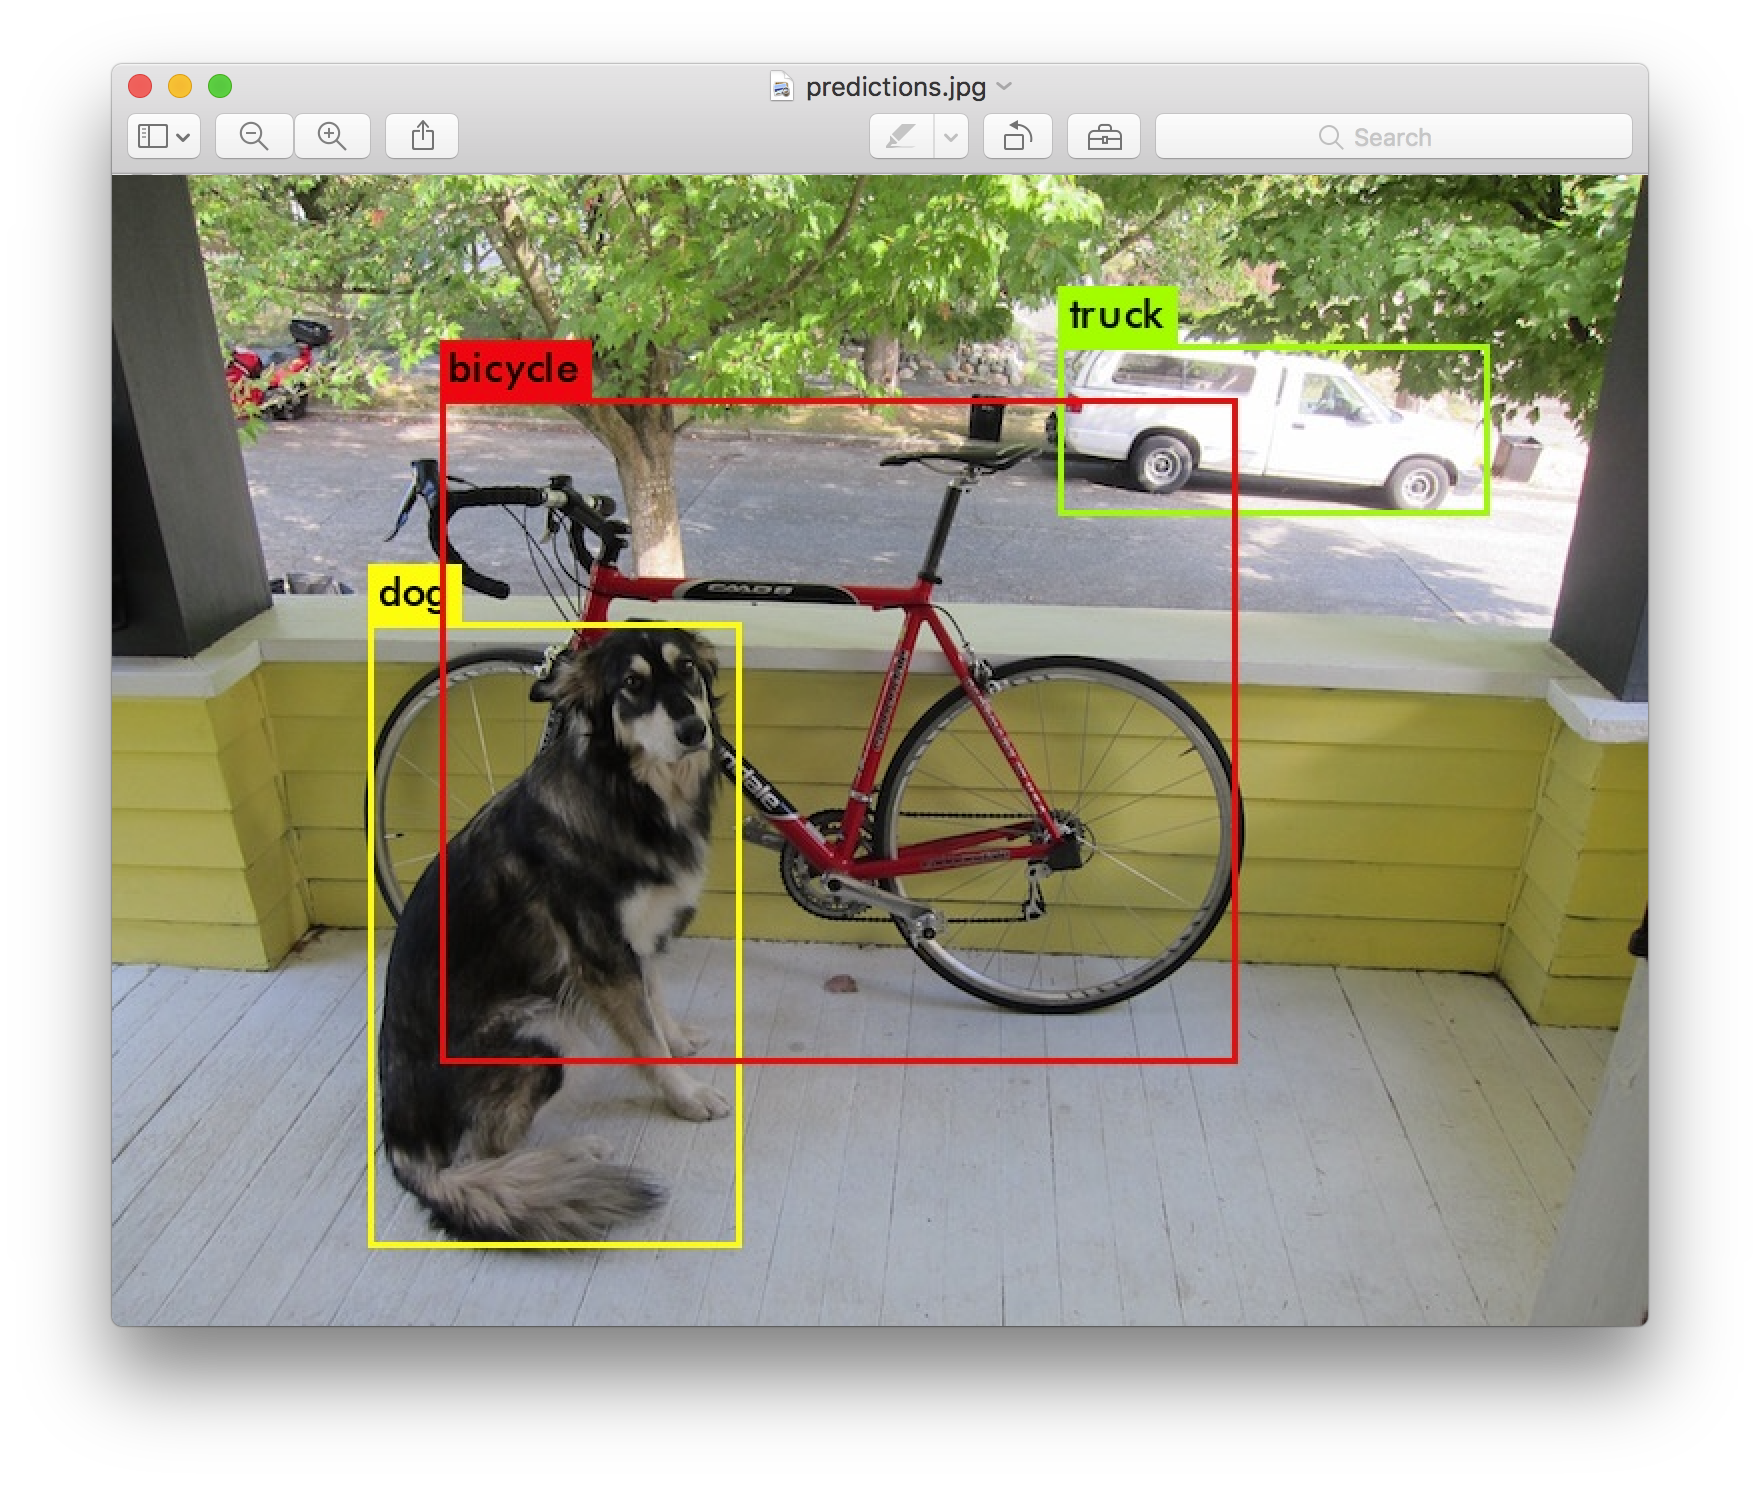
\includegraphics[width=0.5\textwidth]{fig/yolopredictions.png}
    \caption{\label{fig:yolov3}Yolo Predivtions.}
\end{figure}
%指出問題的研究動機:也就是在此研究領域上,有何新研究問題需要被解決? 前人的成果中有那些缺失處或未考慮的因素?或有那一些傳統難題未被徹底解決的?
在卷積神經網路中,目前我們所知若是將神經網路的深度加高,可以提升準確率,但過多的深度卻會造成其效率降低。\\
\begin{figure}[H]
  \centering
    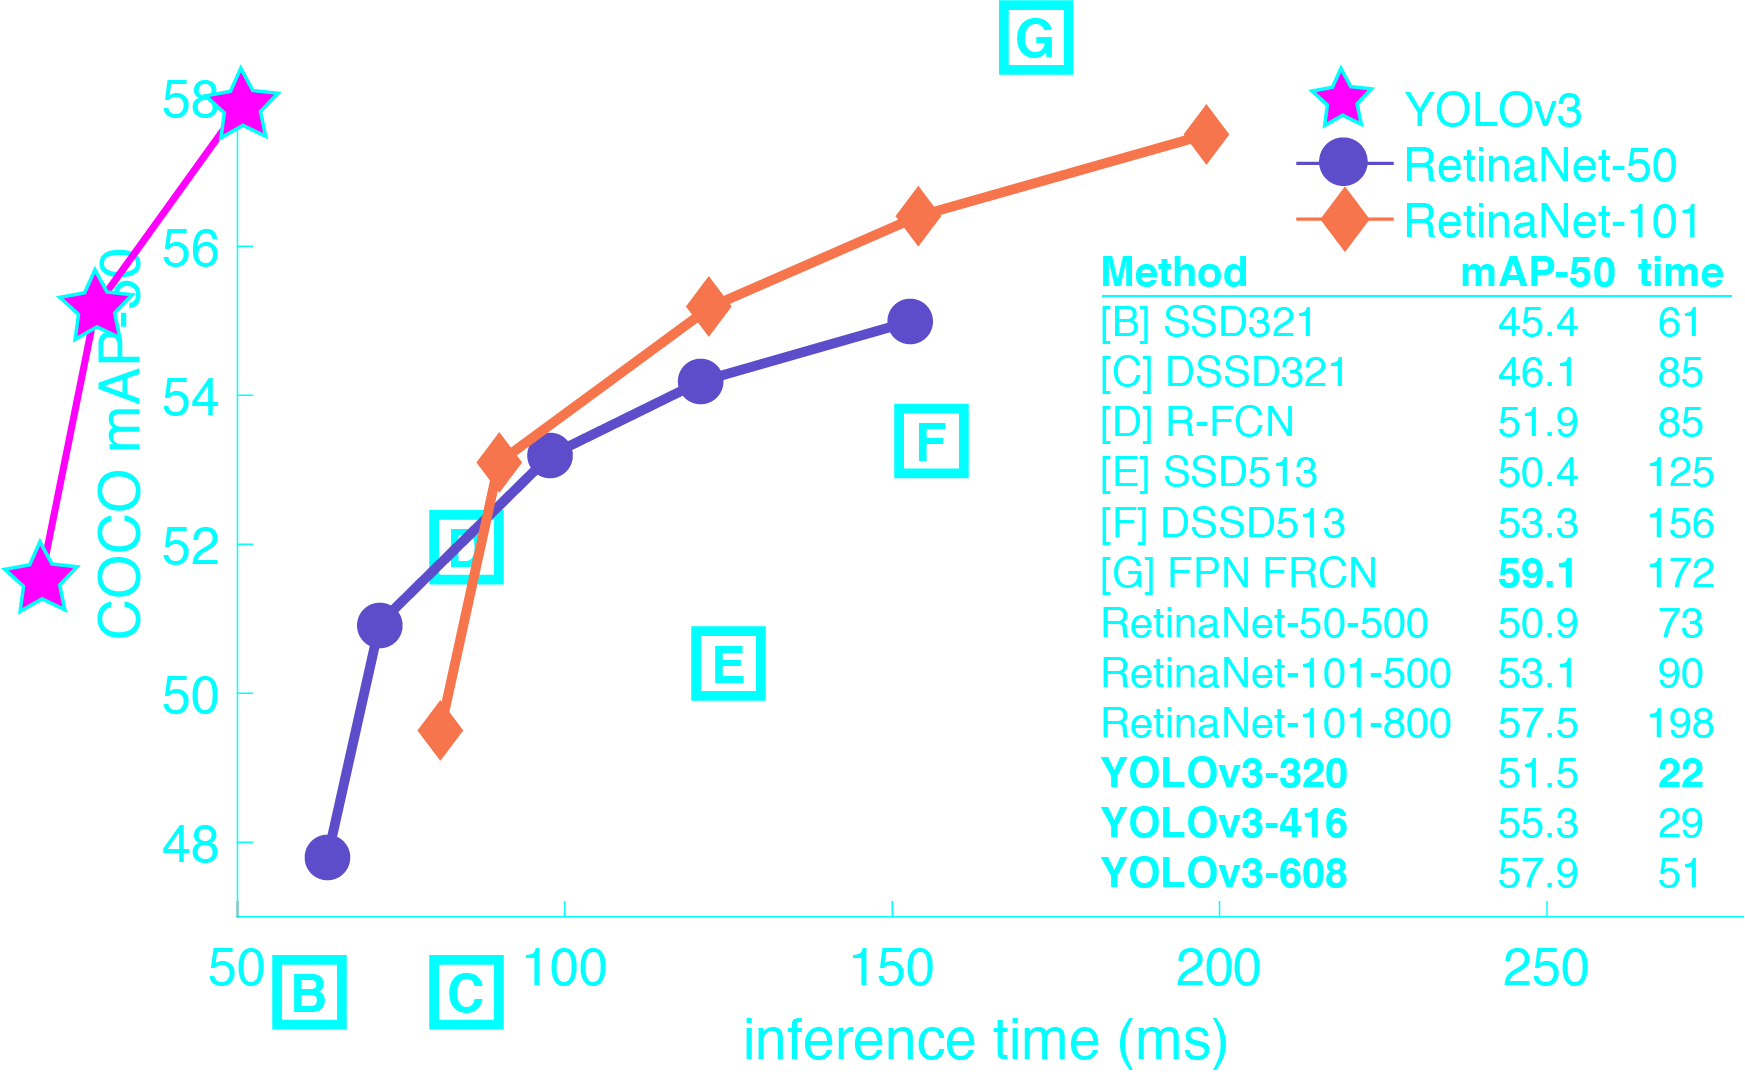
\includegraphics[width=0.5\textwidth]{fig/map50blue.png}
    \caption{\label{fig:yolov3}Yolo v3與其他演算法示意圖.}
\end{figure}
所以現今大部分的演算法只能使用試誤法,以低效率的方式去測驗比較此演算法,粗略估計此演算法的深度與效能達到平衡,常常會有過高的深度或準確率未達預期的情形發生,為了解決此問題,本論文著重於解析卷積神經網路的架構及其運作方法,以簡單明瞭的方式闡述其過程,並且分析原本架構的問題,改善原本的架構。\\

\begin{figure}[H]
\centering  
\subfigure[三分搜尋]{
\label{Fig.sub.1}
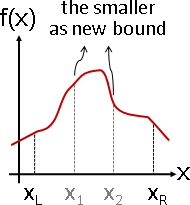
\includegraphics[width=0.45\textwidth]{fig/Optimization4.png}}
\subfigure[總體平均]{
\label{Fig.sub.2}
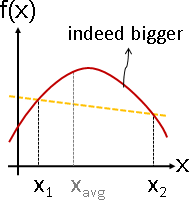
\includegraphics[width=0.45\textwidth]{fig/Optimization5.png}}
\caption{試誤法}
\label{Fig.main}
\end{figure}
%與其他的比較
以往的論文幾乎沒有以視覺化的方式解析卷積神經網路的運作原理,所以在本論文中,希望能以簡單清晰的方式讓人們了解卷積神經網路,並且能在網頁上呈現,其操作性較為直覺性,能夠馬上知道目前選取的位置的功能與效果。
\begin{figure}[htpb!]
  \centering
    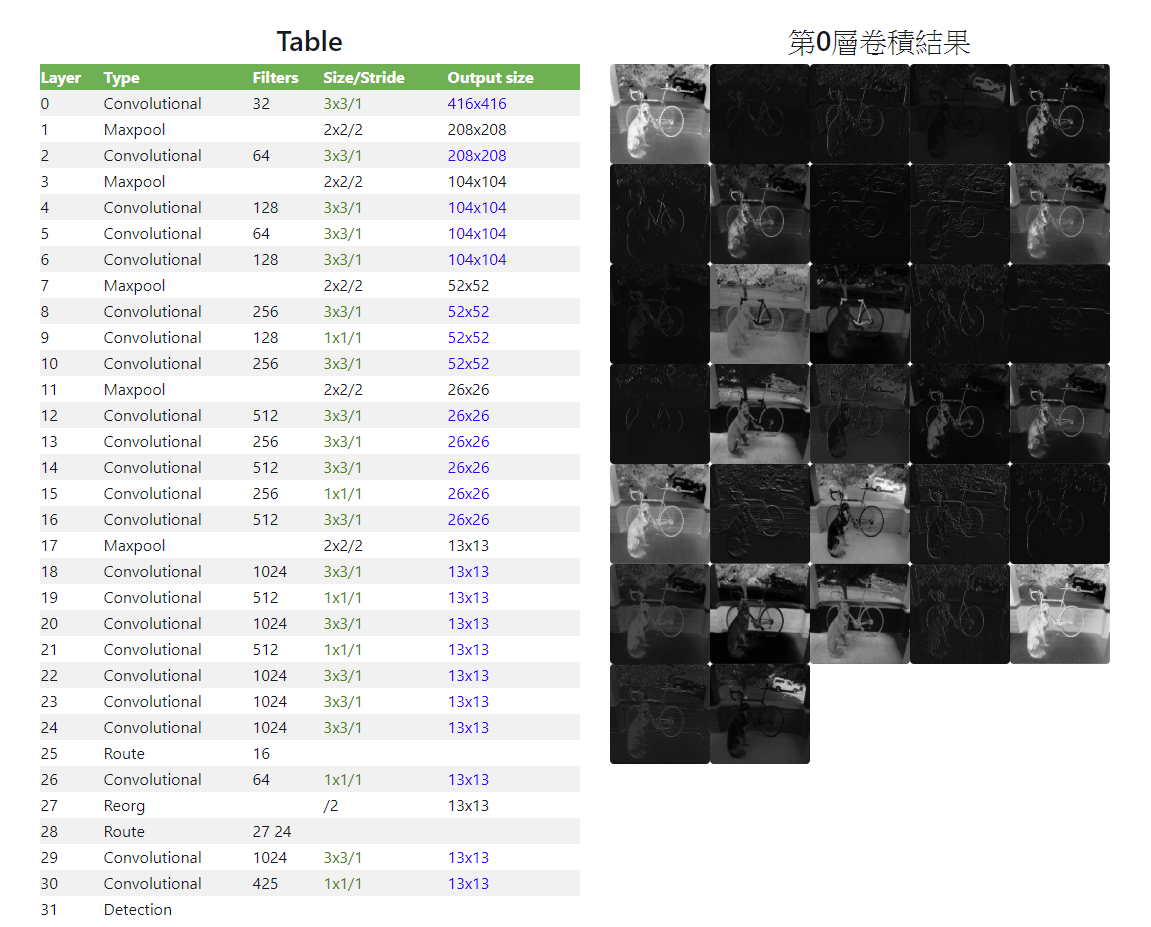
\includegraphics[width=0.5\textwidth]{fig/system1.png}
    \caption{\label{fig:系統1}系統示意圖.}
\end{figure}
%前述的問題期望如何被解決:如降低演算法的時間複雜度或減少電源的耗費或降低網路部署的成本等。儘可能提出明確的方向,如可量化的數量或質性的改善。說明你要解決或是想更進一步瞭解的問題?
\\原本使用Yolo演算法時,必須先完成其環境安裝,並使用程式的指令才能完成其物件偵測。本論文提出一個線上的使用環境,只要將圖片拖曳到網頁中,就可以偵測到其內容出現的物件,大幅改善原本使用的限制。\\

\section{Table}
\label{ss:Table}

 \begin{table}[htpb]\begin{center}
	\label{t:prefix-table}
	\caption{各演算法派別比較}
	\renewcommand{\arraystretch}{1.0}
	\begin{tabularx}{300pt}{|c|X| }
		\hline
		\multirow{1}{*}{\textbf{名稱}} &
		應用範圍
		\\ \hline\hline
		%------------------------------
		\multirow{2}{*}{\textbf{符號論學派}} &
        用逆向演算法,用哲學,心理學, 邏輯思路.
        \\ \hline
		%------------------------------
		\multirow{1}{*}{\textbf{貝氏定理學派}} &
		用機率推理, 用統計學
		\\ \hline
		%------------------------------
		\multirow{2}{*}{\textbf{類比推理學派}} &
		用支持向量機 (support vector machine), 相似度判斷學學習,受新理學,數學最佳化影響
		\\ \hline
		%------------------------------
		\multirow{2}{*}{\textbf{類神經網路學派}} &
		 用大腦逆向工程 (reverse engineering),用倒傳遞理論演算法 (back propagation), 受神經科學,物理學啟發
		\\ \hline
		%------------------------------
		\multirow{2}{*}{\textbf{演化論學派}} &
		 運用遺傳學(genetics), 演化生物學 (evolutionary biology) ,遺傳程式規劃 (genetic programming)
		\\ \hline
		%------------------------------
		
	\end{tabularx}
\end{center}
其中YOLO分類於類神經網路學派,使用卷積神經網路實現物件偵測的網路架構。
\end{table}